%%%%%%%%%%%%%%%%%%%%%%%%%%%%%%%%%%%%%%%%%%%%%%%%%%%%%%%%%%%%%%%%%%%%%%%%%%%%%%%
%                         CAPITULO 3
%                  Redes de Area Local y Encaminamiento
%%%%%%%%%%%%%%%%%%%%%%%%%%%%%%%%%%%%%%%%%%%%%%%%%%%%%%%%%%%%%%%%%%%%%%%%%%%%%%%

\chapter{Redes de Area Local y Encaminamiento}

Hasta ahora hemos estudiado como comunicar dos dispositivos mediante cables
(UART, RS-232) y mediante ondas de radio (Bluetooth, Wi-Fi). Sin embargo, en
un entorno industrial real no hay solo dos dispositivos: hay cientos de
ordenadores, PLCs, sensores, servidores y camaras, todos conectados entre si
y con la necesidad de compartir informacion.

En este capitulo abordamos las \textbf{redes de computadores} desde una
perspectiva arquitectonica: como se organizan fisicamente, como se identifican
los dispositivos, como se toman las decisiones de donde enviar los paquetes de
datos y que dispositivos permiten que una red se conecte con otra.


\section{TCP/IP}

El modelo \textbf{TCP/IP} es la arquitectura de comunicaciones de Internet. En su version simplificada, consta de cuatro capas:

\begin{definicion}
\textbf{IP (Internet Protocol)} es el protocolo que obtiene y define la direccion IP del destino. Actua como un numero de telefono asignado a cada dispositivo en la red.

\textbf{TCP (Transmission Control Protocol)} transporta y enruta los datos a traves de la red, garantizando la entrega al destino que IP ha definido. Es la tecnologia que permite establecer la comunicacion entre dos puntos.
\end{definicion}

\subsection{Capas del modelo TCP/IP}

\begin{itemize}
    \item \textbf{Capa de aplicacion}: protocolos para aplicaciones de red (HTTP, FTP, DNS, SMTP, etc.).
    \item \textbf{Capa de transporte}: transmision de datos entre procesos. Protocolos: TCP (fiable) y UDP (rapido).
    \item \textbf{Capa de Internet (Red)}: direccionamiento y encaminamiento de paquetes. Protocolo: IP.
    \item \textbf{Capa de enlace de datos}: transmision fisica por el medio (cable, fibra, radio).
\end{itemize}

\begin{figure}[H]
\centering
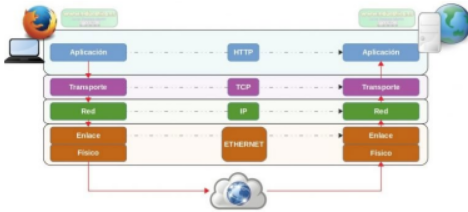
\includegraphics[width=0.8\textwidth]{assets/cap3/3.1.png}
\caption{Pila de protocolos TCP/IP}
\label{fig:pila-tcpip}
\end{figure}


\section{TCP}

\begin{definicion}
\textbf{TCP} (Transmission Control Protocol) es un protocolo de la capa de transporte \textbf{orientado a conexion}. Hace fiable la comunicacion: si falta un paquete o hay error, solicita el reenvio. Solo entrega los datos al nivel superior si estan completos.
\end{definicion}

\begin{figure}[H]
\centering
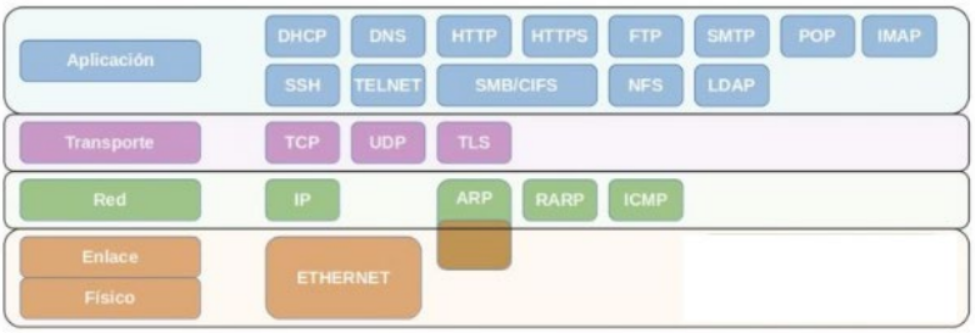
\includegraphics[width=0.8\textwidth]{assets/cap3/3.2.png}
\caption{Funcionamiento de TCP orientado a conexion}
\label{fig:funcionamiento-tcp}
\end{figure}


\section{UDP}

\begin{definicion}
\textbf{UDP} (User Datagram Protocol) es un protocolo de la capa de transporte \textbf{sin conexion}, mas rapido que TCP. No garantiza recepcion ni orden de los datos. Es adecuado cuando la velocidad importa mas que la fiabilidad: juegos en linea, streaming, DNS.
\end{definicion}

\begin{table}[htbp]
\centering
\small
\caption{Comparativa TCP vs UDP}
\begin{tabularx}{\textwidth}{@{}lXX@{}}
\toprule
\textbf{Caracteristica} & \textbf{TCP} & \textbf{UDP} \\
\midrule
Conexion & Orientado a conexion & Sin conexion \\
Fiabilidad & Fiable (reenvia paquetes perdidos) & No fiable \\
Orden de entrega & Entrega ordenada & Sin orden garantizado \\
Latencia & Mayor latencia & Baja latencia \\
\bottomrule
\end{tabularx}
\end{table}

\begin{figure}[H]
\centering
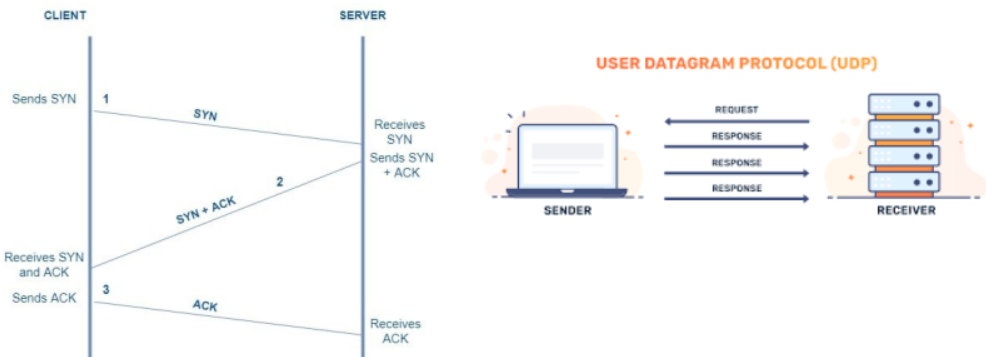
\includegraphics[width=0.8\textwidth]{assets/cap3/3.3.png}
\caption{Comparativa TCP vs UDP}
\label{fig:comparativa-tcp-udp}
\end{figure}


\section{Direccionamiento IP}

Cada dispositivo en una red tiene un \textbf{identificador unico}: la direccion IP. Ademas, cada tarjeta de red dispone de una \textbf{direccion MAC} (Media Access Control), una direccion fisica unica de 48 bits asignada por el fabricante.

\begin{definicion}
Una \textbf{direccion IP} es un identificador numerico que permite localizar un dispositivo dentro de la red y enrutar los paquetes hacia el.
\end{definicion}

\subsection{Representacion IP}

\begin{itemize}
    \item Secuencia de \textbf{32 bits} (4 octetos).
    \item Notacion decimal punteada: \texttt{192.168.1.2}.
    \item Cada octeto: 8 bits, valores de 0 a 255.
\end{itemize}

\begin{figure}[H]
\centering
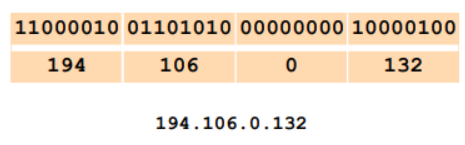
\includegraphics[width=0.8\textwidth]{assets/cap3/3.4.png}
\caption{Formato de una direccion IP de 32 bits}
\label{fig:formato-ip}
\end{figure}

\subsection{IP Dinamica}

Asignada por un servidor \textbf{DHCP} al conectarse. Cambia cada vez que el dispositivo se reconecta. Tipica en hogares.

\subsection{IP Fija}

No cambia. Usada en empresas para identificar servidores, administradores, etc.


\section{Direccionamiento IP con Clase}

Historicamente, las direcciones IP se dividieron en clases. Cada IP tiene dos partes: \textbf{red} y \textbf{host}. Los octetos dedicados a cada una definen la clase.

\begin{figure}[H]
\centering
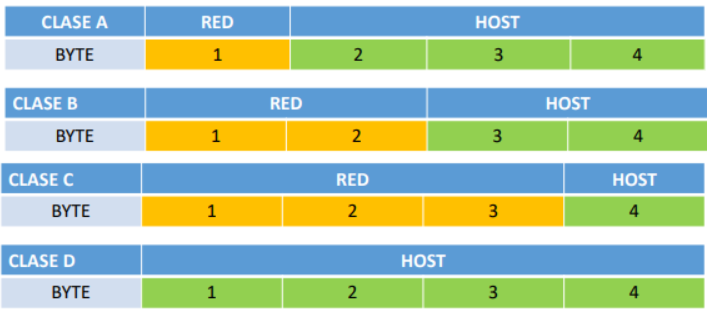
\includegraphics[width=0.8\textwidth]{assets/cap3/3.5.png}
\caption{Estructura de direcciones IP con clase}
\label{fig:ip-con-clase}
\end{figure}

\subsection{Clase A}

\begin{itemize}
    \item Red: 1.\textsuperscript{er} octeto. Host: 3 octetos restantes.
    \item 1.\textsuperscript{er} bit siempre \texttt{0}.
    \item Rango: 1 -- 126.
    \item Hasta ~16 millones de hosts por red.
\end{itemize}

\subsection{Clase B}

\begin{itemize}
    \item Red: 1.\textsuperscript{er} y 2.\textsuperscript{o} octeto. Host: 3.\textsuperscript{er} y 4.\textsuperscript{o} octeto.
    \item 1.\textsuperscript{er} bits siempre \texttt{10}.
    \item Rango: 128 -- 191.
    \item Redes de tamano moderado a grande.
\end{itemize}

\subsection{Clase C}

\begin{itemize}
    \item Red: 1.\textsuperscript{er}, 2.\textsuperscript{o} y 3.\textsuperscript{er} octeto. Host: 4.\textsuperscript{o} octeto.
    \item 1.\textsuperscript{er} bits siempre \texttt{110}.
    \item Rango: 192 -- 223.
    \item Maximo 254 hosts por red. Uso mas frecuente.
\end{itemize}

\subsection{Clase D}

\begin{itemize}
    \item Para \textbf{multicast}: un paquete se envia a un grupo predefinido de IPs.
    \item 1.\textsuperscript{er} bits siempre \texttt{1110}.
    \item Rango: 224 -- 239.
\end{itemize}

\subsection{Clase E}

\begin{itemize}
    \item Reservada para investigacion (IETF).
    \item Rango: 240 -- 255.
\end{itemize}

\subsection{Resumen de clases}

\begin{table}[htbp]
\centering
\small
\caption{Resumen de clases de direcciones IP}
\begin{tabularx}{\textwidth}{@{}lXX@{}}
\toprule
\textbf{Clase} & \textbf{Rango (1.\textsuperscript{er} octeto)} & \textbf{Uso} \\
\midrule
A & 1 -- 126 & Redes muy grandes (~16M hosts) \\
B & 128 -- 191 & Redes medianas (65.534 hosts) \\
C & 192 -- 223 & Redes pequenas (254 hosts) \\
D & 224 -- 239 & Multicast \\
E & 240 -- 255 & Investigacion \\
\bottomrule
\end{tabularx}
\end{table}

\subsection{Direcciones de redes privadas}

\begin{table}[htbp]
\centering
\small
\caption{Direcciones de redes privadas}
\begin{tabularx}{\textwidth}{@{}lX@{}}
\toprule
\textbf{Clase} & \textbf{Rango} \\
\midrule
A & 10.0.0.0 -- 10.255.255.255 \\
B & 172.16.0.0 -- 172.31.255.255 \\
C & 192.168.0.0 -- 192.168.255.255 \\
\bottomrule
\end{tabularx}
\end{table}

\subsection{Direcciones de red y especiales}

\begin{itemize}
    \item \textbf{Direccion de red}: todos los bits de host a 0 (ej. \texttt{113.0.0.0} en clase A).
    \item \textbf{Direccion de difusion (broadcast)}: todos los bits de host a 1.
    \item \textbf{Direccion de multidifusion}: todos los bits de red a 1.
\end{itemize}


\section{CIDR (Enrutamiento sin Clases)}

El direccionamiento \textbf{CIDR} (Classless Inter-Domain Routing) reemplazo el direccionamiento por clases para mayor flexibilidad.

\begin{definicion}
\textbf{CIDR} es un metodo de asignacion de direcciones IP que permite crear redes de cualquier tamano mediante la \textbf{notacion de prefijo}. Por ejemplo, \texttt{192.168.1.0/24} indica que los primeros 24 bits son la red.
\end{definicion}

Ventajas:
\begin{itemize}
    \item Permite crear redes de cualquier tamano, no limitadas a las clases A, B o C.
    \item \textbf{Agregacion de rutas (supernetting)}: una entrada en la tabla de enrutamiento puede representar multiples redes.
\end{itemize}

\subsection{Mascaras comunes}

\begin{table}[htbp]
\centering
\small
\caption{Mascaras de subred comunes en notacion CIDR}
\begin{tabularx}{\textwidth}{@{}lXX@{}}
\toprule
\textbf{Prefijo CIDR} & \textbf{Mascara} & \textbf{Hosts utiles} \\
\midrule
/30 & 255.255.255.252 & 2 \\
/28 & 255.255.255.240 & 14 \\
/24 & 255.255.255.0 & 254 \\
/16 & 255.255.0.0 & 65.534 \\
\bottomrule
\end{tabularx}
\end{table}


\section{DNS (Domain Name System)}

El \textbf{DNS} (Sistema de Nombres de Dominio) traduce nombres de dominio (FQDN) a direcciones IP y viceversa. Tiene una estructura \textbf{jerarquica} y bases de datos \textbf{distribuidas}. Normalmente ejecuta \textbf{BIND} (Berkeley Internet Domain Name).

\begin{definicion}
El \textbf{DNS} es un sistema jerarquico y distribuido que traduce nombres de dominio legibles por humanos (como \texttt{www.upv.es}) a direcciones IP numericas que las redes utilizan para identificar dispositivos.
\end{definicion}

\begin{figure}[H]
\centering
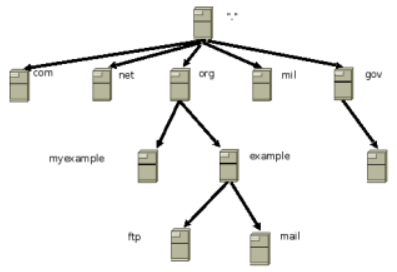
\includegraphics[width=0.8\textwidth]{assets/cap3/3.6.png}
\caption{Jerarquia y funcionamiento del DNS}
\label{fig:dns-jerarquia}
\end{figure}

\subsection{Componentes del DNS}

\begin{itemize}
    \item \textbf{Root Servers}: 13 servidores raiz (A--M), mayoria en USA.
    \item \textbf{TLD Servers}: servidores de dominio de nivel superior (.com, .es, etc.).
    \item \textbf{Authoritative DNS Servers}: servidores autoritativos para un dominio.
\end{itemize}

\subsection{Tipos de resolucion}

\begin{itemize}
    \item \textbf{Consulta interactiva}: el servidor consulta a otros y redirige al cliente.
    \item \textbf{Consulta recursiva}: el servidor resuelve completamente y devuelve la respuesta.
\end{itemize}

\subsection{DNS Internos vs Externos}

\begin{itemize}
    \item \textbf{DNS Interno}: resuelve nombres dentro de una red local (compania). Conoce IPs privadas.
    \item \textbf{DNS Externo / Autoritativo}: visible desde Internet. Solo contiene registros de servicios publicos.
    \item Los DNS autoritativos se configuran al registrar un dominio a traves de un \textbf{REGISTRAR} acreditado por \textbf{ICANN}.
\end{itemize}


\section{DHCP (Dynamic Host Configuration Protocol)}

El \textbf{DHCP} permite la administracion centralizada de la configuracion IP de los dispositivos de una red.

\begin{definicion}
\textbf{DHCP} (Dynamic Host Configuration Protocol) es un protocolo que asigna automaticamente direcciones IP y otros parametros de configuracion (mascara, gateway, DNS) a los dispositivos cuando se conectan a la red.
\end{definicion}

\subsection{Beneficios}

\begin{itemize}
    \item Administracion centralizada de configuracion IP.
    \item Configuracion consistente.
    \item Flexibilidad y escalabilidad.
\end{itemize}

\begin{figure}[H]
\centering
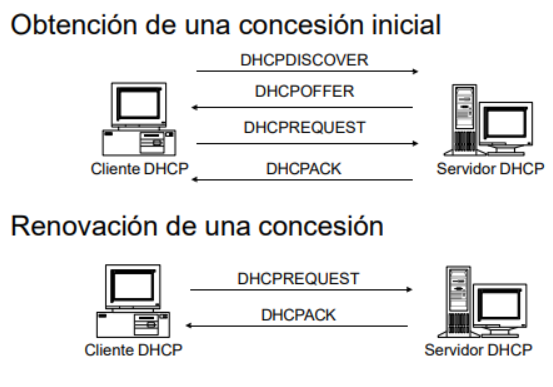
\includegraphics[width=0.8\textwidth]{assets/cap3/3.7.png}
\caption{Funcionamiento de DHCP: proceso DORA}
\label{fig:dhcp-dora}
\end{figure}

\subsection{Funcionamiento: concesion inicial (DORA)}

\begin{verbatim}
Cliente -> DHCPDISCOVER -> Servidor
Cliente <- DHCPOFFER    <- Servidor
Cliente -> DHCPREQUEST  -> Servidor
Cliente <- DHCPACK      <- Servidor
\end{verbatim}

\subsection{Renovacion}

\begin{verbatim}
Cliente -> DHCPREQUEST -> Servidor
Cliente <- DHCPACK     <- Servidor
\end{verbatim}

\subsection{Mensajes DHCP}

\begin{table}[htbp]
\centering
\small
\caption{Mensajes del protocolo DHCP}
\begin{tabularx}{\textwidth}{@{}lX@{}}
\toprule
\textbf{Mensaje} & \textbf{Significado} \\
\midrule
DHCPDISCOVER & El cliente pide una IP \\
DHCPOFFER & El servidor ofrece una concesion \\
DHCPREQUEST & El cliente solicita una concesion especifica \\
DHCPACK & El servidor confirma la concesion \\
DHCPDECLINE & El cliente rechaza la IP ofrecida \\
DHCPNACK & El servidor deniega la concesion \\
DHCPRELEASE & El cliente libera la concesion \\
DHCPINFORM & El cliente pide configuracion adicional \\
\bottomrule
\end{tabularx}
\end{table}

\subsection{Puertos}

\begin{itemize}
    \item Cliente: \textbf{UDP 68}
    \item Servidor: \textbf{UDP 67}
\end{itemize}

\subsection{Metodos de configuracion}

\begin{itemize}
    \item \textbf{Servidores DHCP}: asignan IPs automaticamente.
    \item \textbf{Agentes DHCP de relevo}: reenvian peticiones entre subredes.
    \item \textbf{BOOTP}: protocolo predecesor.
\end{itemize}

\subsection{Ambitos DHCP}

\begin{itemize}
    \item Definen rangos de direcciones IP asignables.
    \item Se pueden excluir direcciones manualmente (routers, firewalls, servidores).
    \item Se pueden crear superambitos combinando multiples ambitos.
\end{itemize}


\section{Practica 4: Cisco Packet Tracer}
\label{sec:practica4}

\subsection{Objetivos}

El objetivo de esta practica es entrar en contacto con el simulador de redes
Cisco Packet Tracer y comprender los conceptos fundamentales de una red de
area local:

\begin{enumerate}
    \item Configurar una red de area local (LAN) con al menos 3 ordenadores y un
    switch, asignando direcciones IP, mascara de subred y gateway.
    \item Verificar la comunicacion entre los ordenadores de la misma LAN
    mediante herramientas como ping.
    \item Crear una segunda LAN con un rango de direcciones diferente.
    \item Interconectar ambas LAN mediante un router, configurando sus interfaces
    de red para que actuen como gateway de cada LAN.
    \item Verificar que los ordenadores de una red pueden comunicarse con los de
    la otra a traves del router.
\end{enumerate}

\subsection{Material utilizado}

\begin{itemize}
    \item \textbf{Software}: Cisco Packet Tracer (simulador de redes Cisco).
    \item \textbf{Hardware simulado}: PCs personales, switches (conmutadores) y
    router (encaminador).
    \item \textbf{Redes}:
    \begin{itemize}
        \item Red 1: 192.168.10.0 / 255.255.255.0
        \item Red 2: 192.168.20.0 / 255.255.255.0
    \end{itemize}
\end{itemize}

\subsection{Desarrollo de la practica}

\subsubsection{Primera parte: configuracion de la LAN 192.168.10.0}

Se diseno una red local con 3 ordenadores personales y un switch. Cada
ordenador se configuro con los siguientes parametros:

\begin{itemize}
    \item \textbf{IP}: en el rango 192.168.10.0 (por ejemplo, 192.168.10.1,
    192.168.10.2, 192.168.10.3).
    \item \textbf{Mascara de subred}: 255.255.255.0 (/24).
    \item \textbf{Gateway}: 192.168.10.254 (direccion que ocupara el router).
\end{itemize}

Se anadieron etiquetas a los ordenadores para identificar su nombre y su
IP. A continuacion, se verifico la comunicacion entre los 3 ordenadores
mediante el comando \texttt{ping}. El resultado confirmo que todos los
ordenadores de la misma red local pueden comunicarse entre si a traves del
switch.

\begin{figure}[H]
\centering
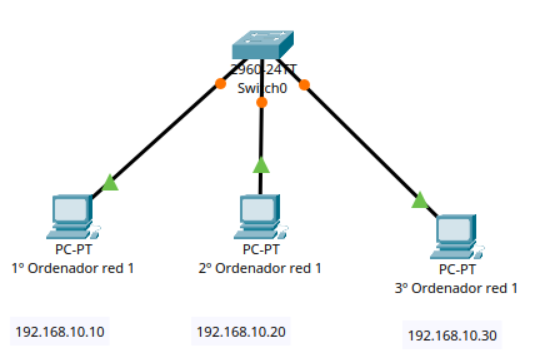
\includegraphics[width=0.8\textwidth]{assets/cap3/3.8.png}
\caption{Topologia de la primera LAN (192.168.10.0)}
\label{fig:lan1}
\end{figure}

\textbf{Comando de verificacion}:
\begin{lstlisting}[language=bash,caption={Verificacion de conectividad en la LAN 1},label={lst:ping-lan1}]
C:\> ping 192.168.10.2

Respuesta desde 192.168.10.2: bytes=32 tiempo<1ms TTL=128
Respuesta desde 192.168.10.2: bytes=32 tiempo<1ms TTL=128
Respuesta desde 192.168.10.2: bytes=32 tiempo<1ms TTL=128
\end{lstlisting}

\subsubsection{Segunda parte: configuracion de la LAN 192.168.20.0 e interconexion}

Se creo una segunda red local con 3 ordenadores mas y otro switch, esta vez
en el rango 192.168.20.0. La configuracion de cada ordenador fue:

\begin{itemize}
    \item \textbf{IP}: en el rango 192.168.20.0 (por ejemplo, 192.168.20.1,
    192.168.20.2, 192.168.20.3).
    \item \textbf{Mascara de subred}: 255.255.255.0.
    \item \textbf{Gateway}: 192.168.20.254.
\end{itemize}

Se verifico que los ordenadores de esta segunda LAN se comunicaban entre si.

\subsubsection{Tercera parte: conexion de ambas LAN mediante un router}

Para que los ordenadores de la red 192.168.10.0 puedan comunicarse con los de
la red 192.168.20.0, se anadio un \textbf{router} entre ambas redes. El router
cuenta con dos interfaces de red (tarjetas), una conectada a cada switch:

\begin{itemize}
    \item \textbf{Interfaz 1}: IP 192.168.10.254 / Mascara 255.255.255.0
    (conectada al switch de la LAN 1).
    \item \textbf{Interfaz 2}: IP 192.168.20.254 / Mascara 255.255.255.0
    (conectada al switch de la LAN 2).
\end{itemize}

Estas dos direcciones son las \textbf{puertas de enlace} (gateway) de cada red.

Se etiquetaron las conexiones del router indicando la red a la que se
conecta cada interfaz y la IP configurada. Finalmente, se verifico la
comunicacion entre ordenadores de ambas redes:

\begin{lstlisting}[language=bash,caption={Verificacion de conectividad entre redes},label={lst:ping-interred}]
C:\> ping 192.168.20.2

Respuesta desde 192.168.20.2: bytes=32 tiempo=1ms TTL=127
Respuesta desde 192.168.20.2: bytes=32 tiempo=1ms TTL=127
Respuesta desde 192.168.20.2: bytes=32 tiempo=1ms TTL=127
\end{lstlisting}

\begin{figure}[H]
\centering
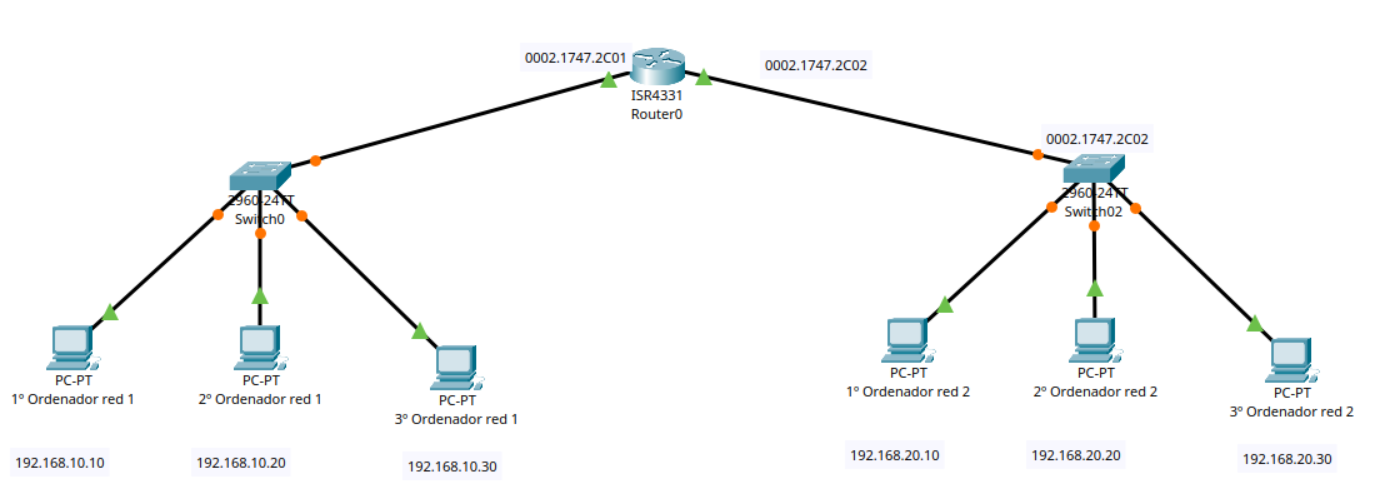
\includegraphics[width=0.8\textwidth]{assets/cap3/3.9.png}
\caption{Topologia completa: interconexion de dos LAN mediante un router}
\label{fig:topologia-completa}
\end{figure}

\subsection{Analisis de la comunicacion entre redes}

Cuando el PC 192.168.10.1 envia un \texttt{ping} al PC 192.168.20.2, ocurre lo
siguiente:

\begin{enumerate}
    \item El PC 192.168.10.1 calcula la red destino aplicando su mascara a la
    IP 192.168.20.2. Detecta que la red destino (192.168.20.0) no coincide
    con su propia red (192.168.10.0).
    \item Por tanto, no puede enviar el paquete directamente. Lo envia a su
    \textbf{gateway}: 192.168.10.254.
    \item El router recibe el paquete por su interfaz 192.168.10.254. Consulta
    su tabla de encaminamiento y detecta que la red 192.168.20.0 es
    \textbf{directamente conectada} a traves de su otra interfaz.
    \item El router reenvia el paquete por la interfaz 192.168.20.254 hacia el
    switch de la LAN 2.
    \item El switch entrega el paquete al PC 192.168.20.2.
    \item El PC 192.168.20.2 responde. Como la IP 192.168.10.1 pertenece a otra
    red, el PC 192.168.20.2 envia la respuesta a su gateway (192.168.20.254).
    \item El router reenvia la respuesta por la interfaz 192.168.10.254.
\end{enumerate}

Este proceso ilustra el concepto fundamental de \textbf{inter-networking}: la
interconexion de redes distintas mediante un dispositivo de capa 3 (router).

\subsection{Relacion teoria-practica}

\begin{table}[htbp]
\centering
\small
\caption{Conexion entre conceptos teoricos y elementos de la Practica 4}
\begin{tabularx}{\textwidth}{@{}lX@{}}
\toprule
\textbf{Concepto teorico} & \textbf{Observacion/aplicacion en la practica} \\
\midrule
Red de computadores & Se disenaron dos redes locales con 3 ordenadores cada una, switch y enlaces fisicos \\
Switch (Capa 2) & Conecta los 3 ordenadores de cada LAN y reenvia paquetes al destinatario correcto \\
Router (Capa 3) & Interconecta las dos LAN distintas, encaminando paquetes entre 192.168.10.0 y 192.168.20.0 \\
Direccion IP & Cada ordenador tiene una IP unica dentro de su rango (192.168.10.x o 192.168.20.x) \\
Mascara de subred & 255.255.255.0 indica que los primeros 3 octetos son red y el ultimo es host \\
Gateway & 192.168.10.254 y 192.168.20.254 son las interfaces del router que actuan como puerta de enlace \\
Comunicacion intra-red & Los PCs de la misma LAN se comunican directamente a traves del switch (ping funciona) \\
Comunicacion inter-red & Los PCs de distintas redes necesitan el router; el ping inter-red confirma el encaminamiento \\
Tabla de encaminamiento & El router internamente tiene una entrada indicando que ambas redes son directamente conectadas \\
Modelo TCP/IP (Capa 3) & El ICMP (ping) opera sobre IP, demostrando la funcion de la capa de red \\
\bottomrule
\end{tabularx}
\end{table}


\section{Resumen de la Unidad 3}

\begin{itemize}
    \item El \textbf{modelo TCP/IP} organiza la comunicacion en cuatro capas: aplicacion, transporte, internet y enlace.
    \item \textbf{TCP} es un protocolo de transporte orientado a conexion y fiable; \textbf{UDP} es un protocolo sin conexion y mas rapido, adecuado para aplicaciones en tiempo real.
    \item Cada dispositivo en una red tiene una \textbf{direccion IP} unica de 32 bits (IPv4), representada en notacion decimal punteada. Puede ser \textbf{dinamica} (asignada por DHCP) o \textbf{fija}.
    \item El \textbf{direccionamiento con clase} (A, B, C, D, E) permite asignar rangos de direcciones segun el tamano de la red. Las \textbf{direcciones privadas} (10.0.0.0/8, 172.16.0.0/12, 192.168.0.0/16) se usan en redes locales.
    \item \textbf{CIDR} reemplazo el direccionamiento por clases mediante notacion de prefijo (ej. /24), permitiendo crear redes de cualquier tamano y agregar rutas (supernetting).
    \item El \textbf{DNS} traduce nombres de dominio a direcciones IP mediante una estructura jerarquica de servidores raiz, TLD y autoritativos.
    \item \textbf{DHCP} asigna automaticamente direcciones IP y configuracion de red a los dispositivos mediante el proceso DORA (Discover, Offer, Request, Acknowledge).
    \item La \textbf{Practica 4} aplica estos conceptos simulando dos LAN conectadas mediante un router en Cisco Packet Tracer, configurando IPs, mascaras, gateways y verificando conectividad con ping.
\end{itemize}
